%% Los cap'itulos inician con \chapter{T'itulo}, estos aparecen numerados y
%% se incluyen en el 'indice general.
%%
%% Recuerda que aqu'i ya puedes escribir acentos como: 'a, 'e, 'i, etc.
%% La letra n con tilde es: 'n.

\chapter{Introducci\'on}
\label{Chapter1} % Change X to a consecutive number; for referencing this chapter elsewhere, use \ref{ChapterX}

%----------------------------------------------------------------------------------------
%	SECTION 1
%----------------------------------------------------------------------------------------

\section{Sistemas polim\'ericos}

En la \'ultima d\'ecada, ha habido un aumento significativo en el inter\'es por los materiales blandos, debido a la amplia variedad y diversidad de materiales e innovaciones que se pueden lograr con ellos. Estos materiales se distinguen por su estructura molecular flexible y adaptable, lo cual les confiere la capacidad de alterar su forma y propiedades de acuerdo con las condiciones externas
Esta adaptabilidad los convierte en protagonistas indispensables en diversas industrias \cite{zhu2022review}. 
Desde su uso en la creaci\'on de espumas y adhesivos  \cite{wu2021review}  hasta su funci\'on prominente como detergentes \cite{chowdhury2019novel}, estos materiales han probado ser efectivos en varios campos. Su aplicaci\'on no se detiene ah\'i, sino que tambi\'en han marcado presencia en la industria cosm\'etica y de pinturas, ofreciendo caracter\'isticas singulares a productos que enriquecen nuestra vida diaria \cite{hirst2019fundamentals}. Incluso en la industria alimentaria, los materiales blandos act\'uan como aditivos esenciales, contribuyendo a la textura, preservaci\'on y seguridad de los alimentos que consumimos \cite{kwok2019microgel}.


Sin embargo, uno de los terrenos m\'as emocionantes en los que los materiales blandos han causado un impacto significativo es en el \'ambito m\'edico y farmac\'eutico \cite{rasool2019stimuli}. Estos materiales se han erigido como protagonistas en la b\'usqueda de transportadores de f\'armacos m\'as avanzados \cite{mcclements2017designing,annabi201425th}, eficientes, amigables con el ambiente y compatibles con el organismo humano. Las propiedades intr\'insecas de los materiales blandos les permiten ser moldeados y adaptados de manera espec\'ifica para cumplir con los requisitos \'unicos de la administraci\'on de medicamentos.
Esta intersecci\'on entre los materiales blandos y la medicina no solo tiene el potencial de revolucionar la forma en que entregamos y absorbemos medicamentos, sino que tambi\'en puede tener un impacto positivo en la calidad de vida de las personas. Tratamientos m\'as efectivos y personalizados que minimizan los efectos secundarios, gracias a la capacidad de estos materiales para interactuar de manera selectiva con el cuerpo humano. Adem\'as, la biodegradabilidad de estos materiales contribuye a la reducci\'on del impacto ambiental, lo que es fundamental en un mundo cada vez m\'as enfocado en la sostenibilidad.
En estas \'ultimas aplicaciones m\'edicas, los films y geles polim\'ericos han sido pioneros en su uso y han tenido un creciente inter\'es. Estos materiales se forman por la uni\'on de cadenas largas de mol\'eculas org\'anicas, es decir pol\'imeros, que pueden tener diferentes grados de entrecruzamiento y solvataci\'on. Los films y geles polim\'ericos tienen la ventaja de poder modificarlos y manipularlos, lo que les permite adaptarse a diferentes necesidades y funciones.
Como resultado, los hidrogeles de pol\'imeros son actualmente candidatos prometedores para el desarrollo de una variedad de biomateriales con aplicaciones en biosensores \cite{zhang2012ultrathin,islam2014responsive}, ingenier\'ia de tejidos \cite{matricardi2013interpenetrating,van2011biopolymer}, regeneraci\'on \'osea \cite{bai2018bioactive}, materiales biomim\'eticos \cite{green2016mimicking,wu2010multifunctional}, entre muchas otras aplicaciones biom\'edicas.

%%%%%%%%%%%%%%%%%%%%%%%%%%
Un \textbf{hidrogel polim\'erico} es un material reticulado en forma de red tridimensional que tiene una alta capacidad de retenci\'on de agua. Est\'a compuesto por pol\'imeros hidrof\'ilicos que absorben y retienen grandes cantidades de agua en su estructura. Los hidrogeles son conocidos por sus propiedades de hinchamiento y absorci\'on de l\'iquidos.
Podemos distinguir entre un  \textbf{un film polim\'erico} el cual consiste en una capa delgada y plana de material polim\'erico que puede tener diferentes espesores. La  matriz de pol\'imeros que la componen se encuentra anclada a la superficie. Los pol\'imeros son cadenas largas de mol\'eculas que pueden ser naturales o sint\'eticas. Los films polim\'ericos se utilizan en una variedad de aplicaciones, incluyendo la construcci\'on, la electr\'onica, y la medicina \addcite.
El film polim\'erico  tiene una alta capacidad de absorci\'on de agua. Como resultado, los hidrogeles polim\'ericos son actualmente candidatos prometedores para el desarrollo de una variedad de biomateriales con aplicaciones en biosensores, ingenier\'ia de tejidos, regeneraci\'on \'osea, materiales biomim\'eticos, administraci\'on de medicamentos y muchas otras aplicaciones biom\'edicas. \cite{Daly2020}

Otras particulas que componen el mundo de los hidrogeles son los \textbf{microgeles}  que al igual que los films definimos anteriormente son redes tridimensionales de pol\'imeros entrecruzados que pueden adsorber grandes cantidades de agua o solventes, lo que les permite hincharse considerablemente. Estos geles tienen dimensiones en una escala de 1 a 200 micrometros. Los microgeles encuentran aplicaciones en \'areas como la ingenier\'ia de tejidos, la liberaci\'on controlada de f\'armacos, la agricultura y la fabricaci\'on de materiales absorbentes. 
En cambio los  \textbf{nanogeles} son estructuras similares a los microgeles, pero su tama\~no se encuentra en la escala nanom\'etrica. Por definici\'on IUPAC este tama\~no debe ser menor a 200 nm \addcite. Los nanogeles son conocidos por sus propiedades de absorci\'on de agua y su capacidad para encapsular mol\'eculas en su interior. Debido a su peque\~no tama\~no y propiedades \'unicas, los nanogeles son ampliamente investigados para aplicaciones biom\'edicas y de entrega de f\'armacos. %% Redundantes (pensar en sacarlo)%%
El entorno acuoso dentro de los hidrogeles puede proteger a las prote\'inas de la desnaturalizaci\'on y agregaci\'on, mientras que estas se mantienen activas y estructuradas cuando se liberan de los hidrogeles. 
En la administraci\'on oral de medicamentos, los hidrogeles con respuesta al pH han sido ampliamente investigados como veh\'iculos funcionales que pueden encapsular y liberar prote\'inas, evitando su degradaci\'on en el entorno gastrointestinal.
Este comportamiento de respuesta es  generalmente reversible y depende de la composici\'on qu\'imica de la red polim\'erica.


\section{Respuesta a estimulo pH, sal y Temperatura}

Los microgeles, compuestos por cadenas polim\'ericas que contienen segmentos \'acidos como el \'acido acrí\'iico o metacr\'ilico (AA y MAA, respectivamente), suelen hincharse o deshincharse en respuesta a cambios en el pH de la solución en la que se encuentran  \cite{snowden1996colloidal}.

\includegraphics[width= 8 cm]{example-image-c} 

El pH en el cual se marca el inicio y caracteriza esta transici\'on es el pKa aparente del microgel, que depende de la concentraci\'on de sal de la soluci\'on y frecuentemente difiere del pKa intrí\'iseco del mon\'omero \'acido.
Estos microgeles tambi\'en ajustan su tama\~no en respuesta a cambios en la concentraci\'on de sal de la soluci\'on \cite{snowden1996colloidal}.
	
An\'alogamente, los microgeles de algunos pol\'imeros termosensibles experimentan una transici\'on de fase de volumen (VPT por sus siglas en ingl\'es) cuando se calientan por encima de una temperatura caracter\'istica (VPTT o $T_{pt}$) \cite{Pelton1986,Pelton2000}.
Este comportamiento se origina porque tales pol\'imeros son insolubles en agua por encima de cierta temperatura de soluci\'on cr\'itica m\'as baja (LCST) \cite{Kawaguchi2020}.
Normalmente, la LCST del pol\'imero y la VPTT de la red  son aproximadamente id\'enticas. 
Este es el caso de las part\'iculas de microgel de poli(N-isopropilacrilamida) (PNIPAm) \cite{Pelton1986}, cuyo volumen colapsa por encima de $32   ^\circ C$, siendo le mismo para el  pol\'imero lineal \cite{Schild1992}.
	
Al tener un VPTT alrededor de la temperatura corporal, los microgeles de PNIPAm han generado un gran inter\'es para aplicaciones biom\'edicas \cite{Guan2011}.
Las estrategias para controlar el VPTT de los microgeles incluyen la s\'intesis de nuevos mon\'omeros termosensibles  \cite{Cai2007,Macchione2019}, as\'i como la copolimerizaci\'on con un mon\'omero i\'onico o ionizable  \cite{Hirose1987,Lopez2020}.
Este \'ultimo enfoque produce microgeles de respuesta m\'ultiple que son susceptibles a cambios en la temperatura, el pH y la concentraci\'on de sal  \cite{snowden1996colloidal, Farooqi2017}.
Los microgeles de NIPAm y AA han sido ampliamente estudiados \cite{Morris1997, Jones2000,Bradley2005,Begum2016};
Tambi\'en se han investigado microgeles de copol\'imeros de NIPAm y MAA  \cite{Dowding2000,Hoare2004,Giussi2015}.
El VPTT de estos microgeles de respuesta m\'ultiple depende del pH de la soluci\'on y la concentraci\'on de sal, y la fracci\'on de mon\'omero ionizable en las cadenas de pol\'imero  \cite{Morris1997,Jones2000, Hoare2004, Bradley2005, Lee2008,Wong2009,Hamzavi2016}.



\section{Encapsulado y Liberaci\'on de medicamentos}

El inter\'es en hidrogeles en especial aquellos con di\'ametros menores a 200 nm ha crecido rotudamente debido a su tiempo m\'as prolongado de circulaci\'on en el sistema circulatorio. La naturaleza incipientemente hidrof\'ilica de estas estructuras, los nanogeles son generalmente biocompatibles y poseen una gran capacidad para incorporar mol\'eculas hu\'esped o analitos, tanto org\'anicos como inorg\'anicos, y prevenir su degradaci\'on por el medio externo. El ambiente acuoso dentro de los hidrogeles puede proteger a las prote\'inas de la desnaturalización y la agregaci\'on [11y13], mientras permanecen activas y estructuradas cuando se liberan de los hidrogeles \addcite[14]. En la administraci\'on oral de f\'armacos, los hidrogeles con respuesta de pH se han investigado en gran medida como veh\'iculos funcionales que pueden encapsular y administrar prote\'inas, evitando su degradaci\'on en el entorno gastrointestinal \addcite[15-17].
Adem\'as, su escaso tama\~no les permite responder r\'apidamente luego de recibir el est\'imulo \cite{tanaka1979kinetics} . Por todas estas razones, los nanogeles polim\'ericos son hoy en d\'ia una de las primeras opciones consideradas al dise\~nar biomateriales con funciones espec\'ificas \cite{soni2016nanogels, sabir2019polymeric}. El est\'imulo que dispara la respuesta de los nanogeles puede ser suministrado por un gradiente en la composici\'on fisiol\'ogica, ya sea natural o inducido por un estado patol\'ogico. La versatilidad de estos materiales dif\'icilmente puede ser alcanzada con otro tipo de nanopart\'iculas, incapaces de responder a cambios en las condiciones del medio que pueden ser relativamente moderados. El desaf\'io en la actualidad es aprender a controlar esta respuesta para canalizarla en diferentes aplicaciones.


Por citar, \citet{Brugger2008} encontraron que el pH durante la s\'intesis tiene un impacto significativo en la composici\'on y, por lo tanto, en las propiedades del microgel y su capacidad para ser utilizado como un estabilizador sensible a est\'imulos.
Resultados similares fueron estudiados por otros autores en donde se destaca el uso de emulsiones sensibles al pH, la sal y la temperatura  \cite{Ngai2005,Ngai2006, Schmidt2011} o como plantillas para el ensamblaje de nanomateriales \cite{Wong2009}.
Haciendo de estos sistema no solo valiosos en el encapsulado y liberaci\'on de medicamentos, sino también como secuestradores de diferentes adsorbatos.

Del mismo modo \citet{Culver2017A}han utilizado nanogeles de poli(NIPAm-co-MAA) funcionalizados para la uni\'on y detecci\'on de diferentes prote\'inas. 
Recientemente se investigaron dispositivos basados en microgeles de poli(NIPAm-co-MAA) para la encapsulación/liberaci\'on del f\'armaco quimioterap\'eutico Doxorrubicina \cite{Giussi2020, MartinezMoro2020, Pergushov2020}. Estos autores mostraron que el uso de microgeles para la liberaci\'on contralada de sustancias bioactivas con carga opuesta. 
La incorporaci\'on del comon\'omero \'acido proporciona un mecanismo controlado por el pH para la captaci\'on/liberaci\'on de mol\'eculas con carga opuesta, lo que hace que los microgeles de respuesta m\'ultiple sean atractivos para el dise\~no de sistemas funcionales de administraci\'on de f\'armacos \cite{Liu2017}.

En s\'intesis el  rango de las potenciales aplicaciones biom\'edicas de los nanogeles es extenso e incluye desarrollos,m\'as especificamente en medicina, contra los trastornos neurol\'ogicos, las enfermedades cardiovasculares, oftalmol\'ogicas, inflamatorias y autoinmunes, as\'i como tambi\'en avances en el diagn\'ostico por im\'agenes, la ingenier\'ia de tejidos, la reconstrucci\'on \'osea y el manejo de la diabetes y el dolor. Por ejemplo, los nanogeles de \'acido hialur\'onico est\'an siendo evaluados para inhibir la acumulaci\'on de la prote\'ina beta-amiloide en el manejo del Alzheimer. En el tratamiento de la diabetes, se investigan nanogeles sensibles a la glucosa y nuevos m\'etodos de administraci\'on de insulina basados en nanogeles.

Los nanogeles de pol\'imeros termosensibles pueden ser utilizados para la administraci\'on localizada de anest\'esicos. Como veh\'iculos para el suministro de drogas, los nanogeles polim\'ericos pueden administrar f\'armacos de peso molecular bajo, oligonucle\'otidos, prote\'inas terap\'euticas e incluso combinaciones de drogas, lo cual es esencial en terapias contra el c\'ancer y las enfermedades infecciosas.

En muchos casos, la v\'ia oral es preferible para la administraci\'on de f\'armacos, ya que es menos invasiva y presenta otras ventajas que mejoran la calidad de vida de los pacientes. En este \'ambito, los nanogeles con respuesta al pH son de particular inter\'es debido a los cambios de pH que ocurren a lo largo del tracto digestivo, desde un medio \'acido en el est\'omago (pH 1.2-2) hasta uno neutro o moderadamente alcalino en el intestino delgado (pH 7-8). Adem\'s, algunos compartimentos celulares involucrados en la captaci\'on de f\'armacos, como los endosomas tempranos, tienen un pH levemente \'acido. La diferencia de pH que existe entre la superficie de la piel  y el torrente sangu\'ineo puede ser aprovechada para la administraci\'on transd\'ermica de f\'armacos utilizando nanogeles con respuesta al pH \addcite[48]. Por otro lado, el microambiente alrededor del tejido canceroso puede presentar un pH m\'as \'acido en comparaci\'on con las condiciones fisiol\'ogicas habituales \addcite[49-52], por lo que los nanogeles con respuesta al pH est\'an siendo evaluados para la administraci\'on de medicamentos en el tratamiento del c\'ancer \addcite[33,53]. Por ejemplo, se han utilizado nanogeles de quitina para la administraci\'on de doxorubicina en diferentes tipos de c\'ancer, incluyendo pulm\'on, mama, h\'igado y pr\'ostata \addcite[54]. Del mismo modo, los nanogeles de pol\'imeros termosensibles tienen un gran potencial para la liberaci\'on dirigida tanto a c\'elulas cancerosas como a tejidos inflamados o lesionados, los cuales presentan una temperatura ligeramente superior a la corporal.
	
En este contexto, esta tesis tiene como objetivo avanzar en el entendimiento de la fisicoqu\'imica que subyace en la actuaci\'on de los geles polim\'ericos como biomateriales y su interacci\'on con prote\'inas y otras biomol\'eculas. Adem\'as, esta investigaci\'on busca explorar nuevas estrategias de funcionalizaci\'on de estos hidrogeles para controlar su respuesta e interacci\'on. Para lograrlo, utilizaremos simulaciones moleculares por computadora, las cuales nos brindan acceso a informaci\'on esencial que a menudo no est\'a disponible en el laboratorio. Al mismo tiempo, el conocimiento adquirido en nuestros estudios tiene como objetivo guiar el dise\~no en el laboratorio de geles polim\'ericos con propiedades \'optimas para aplicaciones espec\'ificas en el campo de los biomateriales.


\section{Enfoque te\'orico}


El control de la funci\'on y el comportamiento de un biomaterial requiere comprender su interacci\'on con las prote\'inas.% Decir más.... tirados de los pelos
 Por ejemplo, las lentes de contacto basadas en \'acido poli(metacr\'ilico) (PMAA) con respuesta al pH est\'an expuestas al fluido lagrimal, que contiene cientos de prote\'inas. La adsorci\'on de algunas de estas prote\'inas debe evitarse, ya que afecta la comodidad de uso y puede provocar inflamaci\'on; sin embargo, la adsorci\'on selectiva de prote\'inas con propiedades antibacterianas y antiinflamatorias, como la lisozima, podr\'ia ser beneficiosa. 
La interacci\'on entre prote\'inas y superficies polim\'ericas est\'a gobernada por una compleja interacci\'on entre diferentes grados de libertad. La capacidad tanto del adsorbato como del material adsorbente para protonar/deprotonar, regular su carga el\'ectrica y modificar el entorno cercano, contribuye a esta complejidad.


El comportamiento de los microgeles de poli(NIPAm-co-MAA), incluido su VPT y la interacci\'on con pol\'imeros de carga opuesta, se ha descrito aplicando teor\'ias  y simulaciones moleculares en varios niveles de resoluci\'on para investigar el comportamiento de los microgeles polim\'ericos sensibles a est\'imulos \cite{ahualli2016coarse,Landsgesell2019SM}.
\citet{quesada2011gel} ha simulado el comportamiento de geles compuestos  polielectrolitos y termosensibles utilizando  simulaciones de Monte Carlo, logrando explicar el comportamiento de hinchamiento de estas part\'iculas.
\citet{ahualli2016coarse}
enplearon simulaciones de grano grueso empleadas para geles polielectrol\'iticos. Este enfoque computacional,se basaron en interacciones part\'icula-partícula entre unidades de pol\'imero. 

En estos trabajos se han centrado principalmente en el hinchamiento y otras propiedades de las part\'iculas que tienen una red de pol\'imero permanentemente cargada , y algunos han abordado el efecto de la temperatura y la calidad del solvente \cite{Jha2011, QuesadaPerez2013, moncho-jorda2016a, ahualli2016coarse, AdroherBenitez2017PCCP}.
Recientemente, estudios  con simulaciones han considerado la respuesta al pH de microgeles compuestos de pol\'imeros reguladores de carga \cite{Schroeder2015,Rud2017,Sean2018, Hofzumahaus2018,Lu2019}.
Sin embargo, solo unos pocos trabajos te\'oricos han investigado las propiedades de los microgeles de respuesta m\'ultiple en funci\'on de la temperatura, el pH y la concentración de sal  \cite{CaprilesGonzalez2008,polotsky2013collapse}.

\citet{polotsky2013collapse} basa su teor\'ia en equilibrios osm\'oticos y teniendo en cuenta expl\'icitamente el equilibrio de ionizaci\'on dentro de sus microgeles. Llegando a predecir patrones complejos en la dependencia de las dimensiones de las part\'iculas de microgel. Es decir sus par\'ametros de control.
	

\section{Antecedentes}

Para estudiar todos los sistemas que presentaremos en cada cap\'itulo, aplicaremos una teor\'ia molecular.
Este enfoque te\'orico permite describir el tama\~no, la forma, la distribuci\'on de carga, el estado de protonaci\'on y la conformaci\'on de todas las especies moleculares que constituyen al sistema. 
Mediante el uso de teor\'ia a nivel molecular, se ha logrado estudiar la termodin\'amica de hidrogeles de cadenas de poli\'acido reticuladas, incluyendo pel\'iculas delgadas depositadas en superficies \cite{longo2012molecular} y pel\'iculas grafteadas en superficies \cite{longo2014non} en estos trabajos se ha investigado el rol que cumple los cambios en el pH y la concetranci\'on de sal respectivamente. En otros trabajos se ha aplicado este marco te\'orico para considerar la adsorci\'on de p\'eptidos y prote\'inas en nanofilmes de hidrogel de cadenas de poli\'acido entrecruzadas \cite{longo2014equilibrium,narambuena2015lysozyme,longo2016adsorption} observadose el trabajo no trivial que tiene el pH al momento de protonar/deprotonar a los distintos adsorbatos. El m\'etodo que usaremos representa una extensi\'on de las teor\'ias moleculares desarrolladas por Szleifer y colaboradores para investigar la adsorci\'on de prote\'inas en capas de pol\'imeros \cite{hagemann2018use,szleifer1997protein,fang2005kinetics}, y el comportamiento de capas de polielectrolitos d\'ebiles \cite{nap2006weak}. Las predicciones de esta teor\'ia se han demostrado estar en excelente acuerdo cuantitativo con observaciones experimentales para una variedad de sistemas polim\'ericos \cite{tagliazucchi2010responsive,wu2007behavior}.
Estos resultados se lograron mediante la formulaci\'on de una energ\'ia libre general que incluye todas las contribuciones relevantes de estos sistemas polim\'ericos: el equilibrio \'acido-base, la p\'erdida entr\'opica de confinamiento molecular, los grados de libertad conformacionales de la red y las prote\'inas (o adsorbatos en general), y las interacciones electrost\'aticas, de Van der Waals y est\'ericas. En estos trabajos se ha buscado comprender c\'omo la adsorci\'on en estas pel\'iculas de hidrogel depende del pH y la concentraci\'on de sal, tanto en soluciones de prote\'inas individuales como en mezclas. En este m\'etodo, el estado de protonaci\'on de los residuos de prote\'inas y de los segmentos de la red no se asume a priori en funci\'on del pH de la soluci\'on (el seno o bulk), sino que se predice localmente como resultado de la posici\'on del grupo y su entorno local. Nuestros estudios resaltan el papel no trivial que desempe\~na la protonaci\'on de los amino\'acidos en la adsorci\'on de prote\'inas. 

En esta secci\'on nos valdremos de una  red polim\'erica que da estructura a un film polim\'erico. Este sistema nos ayudar\'a a introducirnos en la teor\'ia molecular, as\'i como tambi\'en a eplicar algunos concentos que nos ser\'an de suma importancia en los pr\'oximos cap\'itulos.



\section{Metodolog\'ia}

\subsection{Teor\'ia Molecular}

La teor\'ia es un enfoque de funcional de densidad en el cual los campos de interacción se determinan de manera autoconsistente al considerar modelos muy detallados para cada uno de los componentes moleculares del sistema. Obtenemos informaci\'on estructural detallada, as\'i como propiedades termodin\'amicas. En particular, es posible mostrar el fuerte acoplamiento que existe entre el estado termodin\'amico y la estructura del sistema. De esta manera, se puede estudiar c\'omo las variaciones en las condiciones de la soluci\'on, por ejemplo, la fuerza i\'onica y el pH, entre otros, cambian las propiedades termodinámicas.
Para tal fin se usa  una descripci\'on molecular de grano grueso de las diferentes especies qu\'imicas que componen el sistema.
Dicha descripci\'on incluye forma, tama\~no, distribuci\'on de carga (si los hubiese) y estado de protonaci\'on de cada componente molecular en los casos que corresponda.

La teor\'ia se deriva al escribir la energ\'ia libre del sistema como un funcional de las densidades de las especies en soluci\'on, las conformaciones (en esta tesis de la red polim\'erica) y el potencial electrost\'atico, considerando expl\'icitamente los equilibrios \'acido-base . 
Conocer la energ\'ia libre total del sistema es la que nos permite explicar toda la fisicoqu\'imica del sistema.  La minimizaci\'on de esta energ\'ia respecto a la funcional de las densidades permiten obtener el estado de menor energ\'ia que estabiliza al sistema.

En el esquema de la figura \ref{fig:met:tm_esquema} se puede observar como se interpreta esta teor\'ia. Para dicho esquema se ha considera un sistema con una red polim\'erica que posee mon\'omeros titulables, as\'i mismo un adsorbato con unidades qu\'imicas titulables. Esto nos proporciona una energ\'ia libre qu\'imca ($F_{qca}$)dada por los equilibrios \'acido-base.
Adem\'as si consideramos nuestra red polim\'erica como punto de referencia fijo obtenemos una entrop\'ia de mezcla ($S_{mez}$) dada por las especies moviles: mol\'eculas de agua, iones de sal, adsorbatos. Adem\'as hay otra entro\'ia de mezcla dada por las diferentes configuraciones a las que puede acceder la red polim\'erica, es particular la denominamos $S_{conf,net}$.
Otro tipo de interacciones que se incluyen en este ejemplo son las interacciones entre todas las especies. Interacciones del tipo electr\'ostatico ($U_{elec}$) e interacciones est\'ericas ($U_{ste}$) en donde hay restricciones sobre el volumen, todo el espacio debe estar ocupado y no pueden existir superposiciones entre especies. 
Estas contribuciones son funcionales de otras funciones como lo son el grado de carga, las densidades locales de cada especie, potencial electr\'ostatico y una presi\'on osm\'otica. En conjunto lo que se obtiene es un semi-gran potencial. Esto debido que hemos considerado como referencia a la red polim\'erica y no puede desplazarse, sin embargo las especies si crean un equilibriio qu\'imico entre el bulk de la soluci\'on y las cercanias (y dentro) de nuestra red polim\'erica.

La minimizaci\'on de este potencial energ\'etico nos permite escribirlo en funci\'on de dos potenciales de interacci\'on locales. En cada cap\'itulo daremos la derivaci\'on detallada y como es posible llegar a estos potenciales. 
Finalmente la resoluci\'on n\'umerica de estos poteniales se hace con el m\'etodo de Newton-Krylov \cite{brown1994convergence} implementado en c\'odigo FORTRAN escritos en el grupo de investigaci\'on.
 \begin{figure}[!htb]
	\centering
	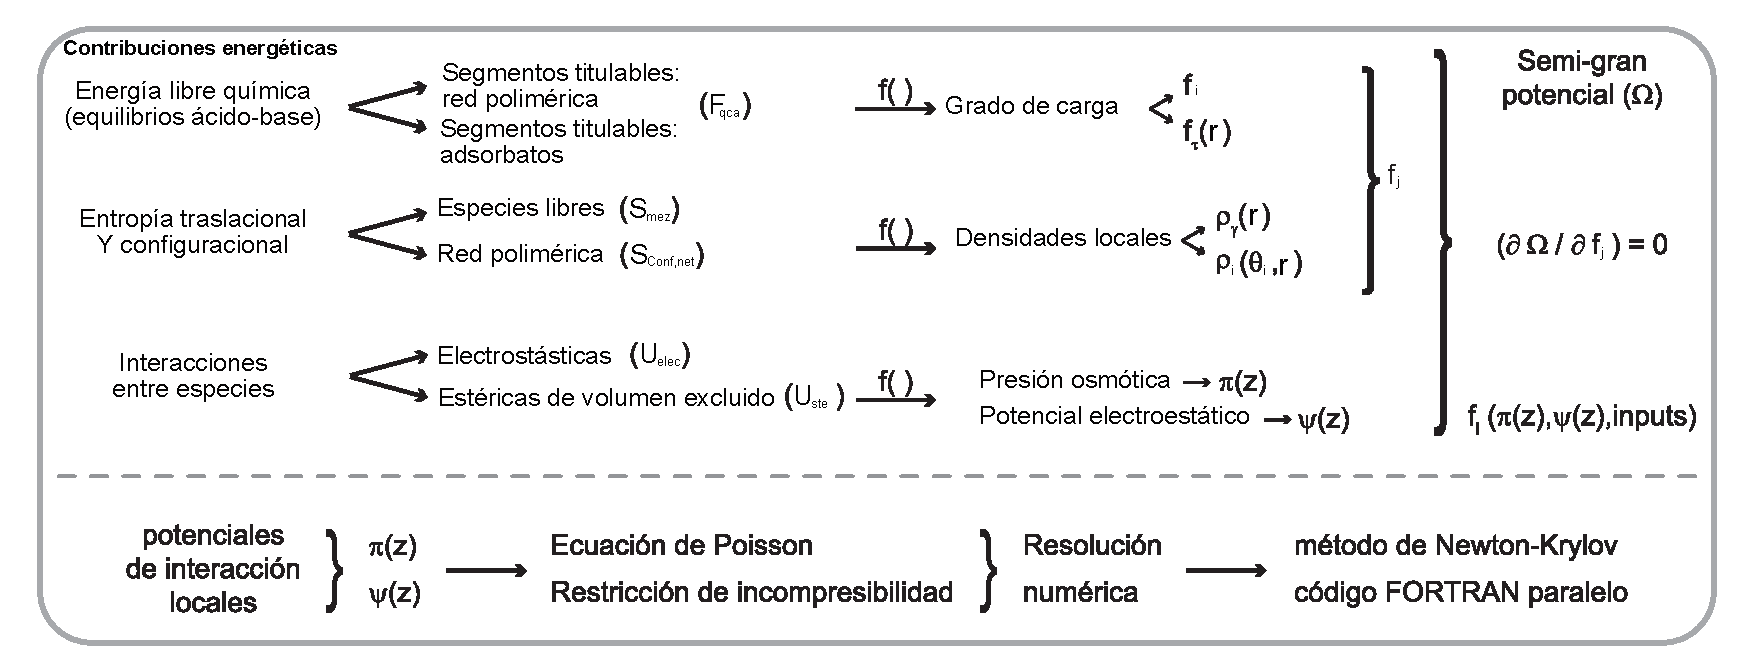
\includegraphics[width=0.99\textwidth]{Figures/TM.pdf}
	\caption{Esquema de la teor\'ia molecular... las diferentes contribuciones energ\'eticas son un funcional de funciones de densidad}
	\label{fig:met:tm_esquema}
\end{figure}


\subsection{Monte Carlo}

El algoritmo Metropolis-Hastings es un m\'etodo de muestreo de Monte Carlo en cadena de Markov (MCMC)  para obtener muestras de una distribuci\'on de probabilidad a partir de la cual es dif\'icil obtener muestras directamente. El algoritmo fue propuesto por Nicholas Metropolis, Walter Wolfgang Gibbs, Geoffrey Hastings, y Ronald L. Tanner en 1953. \cite{metropolis1953rosenbluth}
El proceso Metropolis-Monte Carlo consiste en los siguientes pasos:


\begin{itemize}
	

\item Inicializaci\'on: Se comienza con una configuraci\'on inicial del sistema que puede ser generada aleatoriamente o de alguna otra manera relevante para el problema en cuesti\'on.

\item Perturbaci\'on: Se genera una nueva configuraci\'on perturbando la configuraci\'on actual. Esto puede realizarse mediante cambios aleatorios peque\~nos en las posiciones, orientaciones u otras propiedades de las part\'iculas o componentes del sistema.

\item C\'alculo de la Energ\'ia: Se calcula la energ\'ia del sistema para la nueva configuraci\'on y la configuraci\'on actual. La energ\'ia puede incluir t\'erminos potenciales, cin\'eticos y/o interacciones entre componentes.

\item Comparaci\'on de Energ\'ias: Se compara la energ\'ia de la nueva configuraci\'on con la energ\'ia de la configuraci\'on actual. Si la energ\'ia disminuye, la nueva configuraci\'on se acepta autom\'aticamente. Si la energ\'ia aumenta, se calcula una probabilidad de aceptac\'on basada en la diferencia de energ\'ia y una temperatura ficticia. Esta probabilidad introduce una componente estoc\'astica en el proceso, permitiendo la exploraci\'on de configuraciones de mayor energ\'ia.

\item Decisi\'on de Aceptaci\'on: Se genera un n\'umero aleatorio y se compara con la probabilidad de aceptaci\'on. Si el n\'umero aleatorio es menor que la probabilidad de aceptaci\'on, la nueva configuraci\'on se acepta; de lo contrario, se mantiene la configuración actual.

\item Iteraci\'on: Los pasos 2-5 se repiten muchas veces para generar una secuencia de configuraciones. Estas configuraciones forman una muestra estad\'istica del espacio configuracional, lo que permite el an\'alisis de propiedades del sistema.

\item An\'alisis: Utilizando la secuencia de configuraciones generadas, se pueden calcular propiedades macrosc\'opicas del sistema, como promedios de energ\'ia, densidades, funciones de distribuci\'on, entre otras.
\end{itemize}

El algoritmo Metropolis-Hastings es un m\'etodo general que puede ser utilizado para muestrear de una amplia variedad de distribuciones de probabilidad. Es un m\'etodo eficiente y robusto, y se ha utilizado en una amplia variedad de aplicaciones, incluyendo f\'isica, qu\'imica, biolog\'ia, econom\'ia, y finanzas.\cite{sin2020applications}

\subsection{Dinamica Molecular}

La din\'amica molecular (MD) es una t\'ecnica computacional que permite estudiar el comportamiento de las mol\'eculas a trav\'es del tiempo. Esta t\'ecnica simula el movimiento de los \'atomos que componen las mol\'eculas, y permite observar c\'omo las mol\'eculas interact\'uan entre s\'i y con su entorno.
GROMACS es un software de c\'odigo abierto que se utiliza para realizar simulaciones de din\'amica molecular. \cite{lindahl2001gromacs}
El paquete de simulaci\'on GROMACS es ampliamente utilizado para llevar a cabo simulaciones de din\'amica molecular en sistemas biol\'ogicos, qu\'imicos y materiales. Su capacidad para modelar la interacci\'on entre part\'iculas y representar fuerzas realistas permite el estudio de sistemas complejos y la obtenci\'on de resultados cuantitativos y cualitativos significativos.

Esta metodolog\'ia la usaremos para la generaci\'on de configuraciones descrita el en el anexo \ref{anexo-configuraciones}.




%%%%%%%%%%%%%%%%%recorte
%%%%%%%%%%%%%%%%%%%%


%-----------------------------------
%	SUBSECTION 1
%-----------------------------------
\section{Objetivos}

Los {\bf objetivos específicos} del presente plan de trabajo son los siguientes:
%
\begin{enumerate}
\item Desarrollar un modelo mecano-estadístico utilizando TM para describir la respuesta a cambios de pH, temperatura y concentración de sal en microgeles formados por homopolímeros.%\label{objetivo_1}
\item Extender dicho modelo para investigar el comportamiento de microgeles de copolímeros con respuesta a múltiples estímulos.%\label{objetivo_2}
\item Estudiar los mecanismos de adsorción de diferentes biomoléculas en los microgeles en función de las condiciones del medio y la estructura/composición química de las cadenas poliméricas.%\label{objetivo_3}
\item Desarrollar un modelo combinando simulaciones de TM y Dinámica Molecular (DM) para estudiar el comportamiento de estos microgeles en soluciones relativamente concentradas.%\label{objetivo_4}
\end{enumerate}
%

Finalmente el \textbf{objetivo general} de esta tesis consiste en \emph{desarrollar una descripción comprensiva del comportamiento y respuesta a estímulo de los microgeles poliméricos mediante el uso de modelos teóricos y computacionales basados en las interacciones moleculares.}
